\documentclass[a4paper, 12pt]{article}
\usepackage{comment} % enables the use of multi-line comments (\ifx \fi) 
\usepackage{lipsum} %This package just generates Lorem Ipsum filler text. 
\usepackage{fullpage} % changes the margin
\usepackage{bm}
\usepackage{graphicx}
\usepackage{blindtext}
\usepackage{listings}
\usepackage{amsmath}
\usepackage{setspace}
\usepackage[colorlinks=true, linkcolor=black,urlcolor  = black]{hyperref}
\linespread{1.5}
\begin{document}
%Header-Make sure you update this information!!!!
\noindent
Cmpsci585\\
Final Report\\
Patrick Carron \\
Raymond Zhu\\
12/20/2016 \\
\begin{center}

\textbf{Predicting Political Party Affiliation from Speech}
\end{center}

\section{Abstract}
We attempt to classify a speaker's party affiliation from their word usage by analyzing a corpus of congressional speeches.  We investigate the impact of different preprocessing techniques on accuracy and test Multinomial Naive Bayes and Stochastic Gradient Descent classifiers. We preform 3-fold cross-validation on each classifier to find optimal hyper-perameters. We find that bigram language modeling with Tf-Idf weighting and a Stochastic Gradient Descent classifer with Hinge loss, $l2$ regularization penalty, regularization constant $\alpha=.0001$ result in an optimal observed test accuracy of 74.9\%.
	
	\section{Introduction}
	
	This research attempts to predict a speaker's political party affiliation based on the language used in their congressional speeches. We are using the \href{http://www.cs.cornell.edu/home/llee/data/convote.html}{Congressional speeches dataset} created by Lillian Lee at Cornell \cite{thomas2006get}. The dataset has been preprocessed somewhat and split into train, validation, and test sets.  We first perform exploratory data analysis to ensure high data quality and understand some idiosyncrasies of this data asset. We look at differences between the parties in commonly used terms for insight into differences in policy positions. We then use the \cite{pedregosa2011scikit} Scikit Learn library to create a data analysis pipeline to ensure that we have consistency in how the data is being processed while testing both Multinomial Naive Bayes and Stochastic Gradient Descent classifiers.  For each we use 3-fold cross validation to search for optimal hyper-parameters and optimal pre-processing techniques.  We compare cross validation accuracy between unigram and bigram language models and also train our classifiers both including Tf-Idf weighting and excluding Tf-Idf weighting. Ultimately we found that Stochastic Gradient Descent with Hinge loss, $l_2$ penalty, $\alpha=.0001$,  Bigram language modeling with Tf-Idf included gave us the highest test accuracy at 74.9\%.
	
\section{Related Works}
\label{gen_inst}
The first research preformed on this corpus was \cite{thomas2006get} \textbf{Get out the vote: Determining support or opposition from Congressional floor-debate transcripts} by Thomas et al.. In this work they wanted to determine whether a transcript from U.S. Congressional floor debates was supporting or opposing a proposed legislation. In their approach they used an SVM classifier on individual documents using unigrams as features, though in our case our cross validation selected the bigram language model for all classifiers that we experimented with. For the cases of the same speaker they implemented weighted links to allow for "soft" preferences. These "soft" preferences were to show changes in a speaker's opinion over time during the debate. Hard assignments later on in the evaluation proved that "soft" preferences were preferred over hard assignments, in which all labels of that speaker is the same. In this approach they utilized speech-segment relationships in their classification. \\

\noindent	
In \cite{yu2008classifying} \textbf{Classifying Party Affiliation from Political Speech} by Yu et al.. each document is mapped to a vector of word frequencies, and stop words are selected based on high and low frequency thresholds and removed from the document. Then use Naive Bayes and SVM algorithms to train ideology classifiers, and then use leave-one-out cross validation as well as hold-out tests for the evaluation. What they did differently from our approach was that they tested their classifier's time dependency and person dependency. They also tested whether or not they can train on one party data and then use the model to test it on the other party's data, this can be seen when they trained on the House and then tested on the Senate and the other way around. Instead we took an overall dataset and made our model predict labels for an overall data set.\\

\noindent
Finally, In  \cite{iyyer2014political} \textbf{Political Ideology Detection Using Recursive Neural Networks} Iyyer identifies ideological bias within individual sentences within this corpus. In their work instead of using Naive Bayes and SVMs they use Recursive Neural Networks. Also, instead of analyzing a speech, such as in our approach, they analyzed on the sentence-level. This approach also does not follow the usual bag-of-words models that political classification usual has. Using their RNN model they could even detect bias in complex sentences that their baseline using bag-of-words couldn't. 
	

	
\section{Data}
Some preprocessing was already done on the data set to easily parse the speeches in the data set. Each token was forced to lower case and spaces were made around punctuation marks in order to count them as separate tokens. There are some exceptions to this, such as the token ``mr.'', which uses the period as part of the token. Congressional names have also been stripped from the text and replaced with unique identifiers. Each filename within the data set also has information about the speech, and to our interest it includes the political party affiliation of the speaker. We parse the file name to record the party affiliation of each speech, which would serve as our labels for both the training and test data sets. Due to our data set being originally for a research done to classify support or opposition, the documents of the data set are organized around proposed legislation to some speaker voting for or against the bill. Some basic statistics about this data set is that the training corpus composed of 6,362 documents containing 1,544,279 tokens with a vocabulary size of 24,564 terms. The test set is composed of 1,759 documents. The development set that was originally included with the data set was added onto the training set because we use 3-fold cross validation instead of a train, validation, test split. For both the data sets, the contents of the document and its respective labels were recorded through the same method.\\ 

\noindent
As a quality check we looked see that  Zipf's law holds for our data set and also checked high and low frequency terms. We created log scaled Zipf's law representation in \autoref{fig: zip}.This visualization met the expectations, and gave us confidence that our data set is of good quality. The highest terms were largely contractions and determiners, while the single frequency terms seem to be proper nouns or rarely used verbs which matched our expectations. With our documents read in and a high level of confidence in the quality of our data set and representation, we proceeded to implement a data pipeline and perform baseline experiments on our corpus.\\\
\begin{figure}[!ht]
\centering
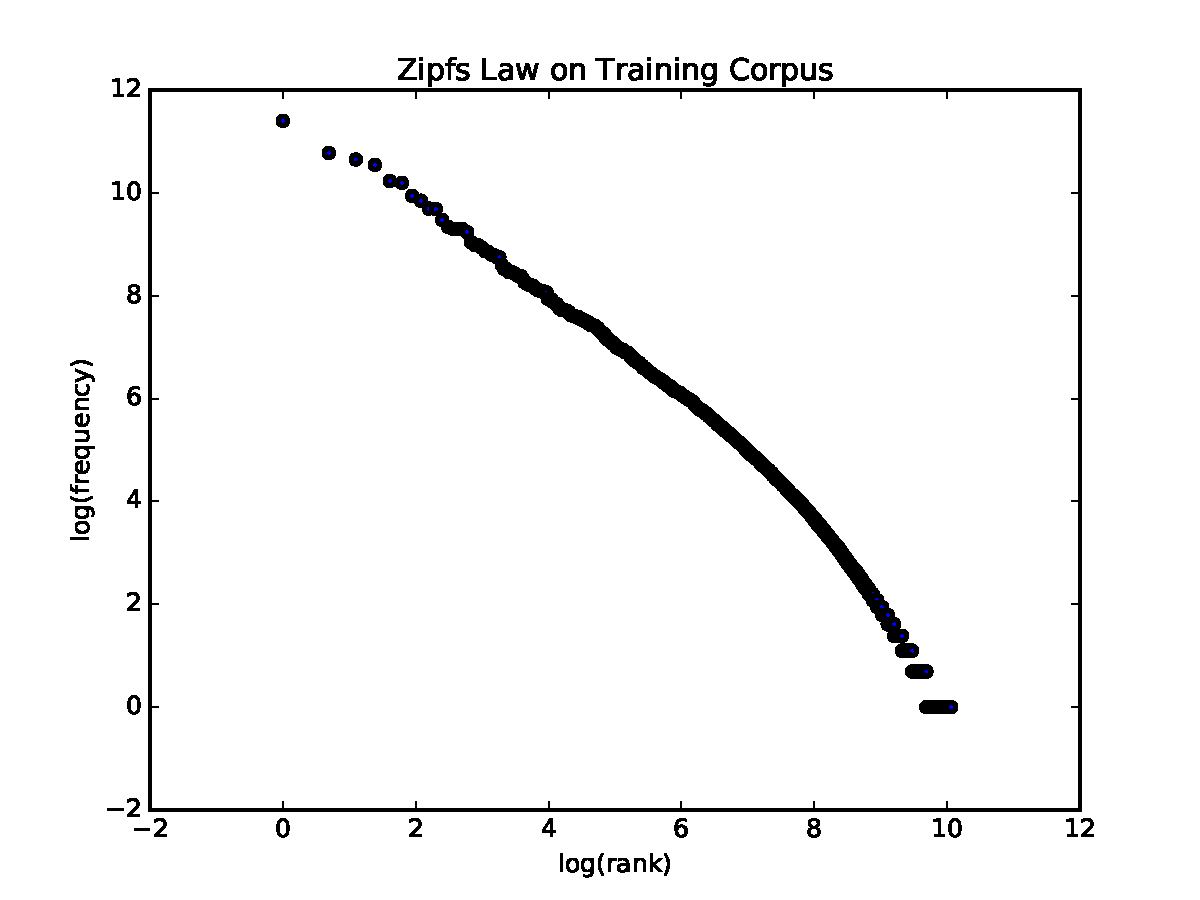
\includegraphics[width=0.5\linewidth]{zipfslaw.pdf}
\caption[Zipf's Law]{Zipf's Law}
\label{fig: zip}
\end{figure}

\noindent

\begin{table}[h]
\centering
\label{Most and Least Common Words}
\begin{tabular}{|c|c|c|c|c|}
\multicolumn{2}{c}{Most Common} & \multicolumn{2}{l}{Least Common (a subset)} \\
\hline
Word                 & Frequency        &  Word & Frequency      \\
\hline
the                  & 89452                & herzog &1\\
to                  & 47827                 &   alfonso &1\\
of                    & 42111                  & thimerosal&1\\
and                   & 37916                    & nehf&1\\
that            & 27776                   & maize&1\\
in                   & 26750                   & dearth&1\\
is                   & 20759                   &hulshof&1\\
this                    & 18897                   & boor&1\\
for                   & 16213                    &eneryville& 1\\
we                & 16039                 & nassau & 1 \\
\hline
\end{tabular}
\end{table}
\noindent
\subsection{Term Differences by Party}
We split the corpus by party affiliation and analyzed the word frequencies for each party to create lists of most frequently and least frequently used terms for each. While there were many common terms like determiners, prepositions and conjunctions, there were some interesting differences. Democrats used terms affiliated with education, healthcare, and energy much more frequently than Republicans in our corpus. 

%\begin{figure}[!ht]
%\centering
% \includegraphics[width=0.5\linewidth]{playerClusters.pdf}
% \caption{Sum of Squares Within Clusters for k=1 to 20}
%\label{fig:cluster}
%\end{figure}


\section{Method}
We use \cite{pedregosa2011scikit} Scikit Learn to create identical data preprocessing pipelines for both our Multinomial Naive Bayes and Stochastic Gradient Descent classifiers.  Since the corpus is comprised of a high volume of terms and documents we select a sparse representation using the CountVectorizer function which allows dictionaries containing tokens as keys and frequencies as values to represent each document in the corpus. We include a Tf-Idf transform in the data pipeline as well. These functions allow us to search across a range of options for preprocessing and look at their impact on cross validation accuracy.  For CountVectorizer we search both Unigram and Bigram language model counting. For the Tf-Idf transform we compare accuracy including the option and excluding the option. This allows us to search for an optimal preprocessing methodology. The classification function is the final method included in the data pipeline and these methods and their hyper-parameters are the only distinguishable characteristic for each experiment allowing us to compare the impact of each classification technique. First we test each classifier using default settings. Then we preform an exhaustive grid search utilizing 3-fold cross validation to find each classifiers respective optimal hyper-parameters with optimal preprocessing to obtain our highest achievable test accuracy. \\

\section{Proposed Solution and Experiments}
\subsection{Optimal Preprocessing}
\subsubsection{Unigram vs. Bigram Language Model}
For each classifier we will compare unigram language modeling against bigram language modeling. Both of these language models are considered to be bag of words models meaning that positional information is largely ignored and documents are viewed as frequency counts of terms. Unigram language modeling is based strictly on the counts of each term in each class whereas bigram language models include counts for terms following other terms. This means that bigram language models count term frequencies along with the frequencies with which each word follows a preceding term. Essentially bigram counting allows for conditional probabilities to be calculated conditioning on a given previous word.  We will compare 3-fold cross-validation accuracies for our models using both unigram and bigram counts to find which results in higher accuracy.
\subsubsection{Tf-Idf Weighting}
When Tf-Idf weighting is included in preprocessing, term frequencies are adjusted by their inverse document frequencies. Scikit learn \cite{pedregosa2011scikit} describes this mathematically as: 
\[tf-idf(t,d)=tf(t,d)idf(t)\]
Where $tf(t,d)$ is the term frequency in a document and $idf(t)$ is the inverse of the number of documents containing the term $t$ in the corpus which is represented as:
\[idf(t)=\log(\frac{1+n_d}{1+df(d,t)}) +1\]
Here $n_d$ is the total number of documents in the corpus and $df(d,t)$ is the count of documents including the term. When inverse document frequency is included, high frequency terms like determiners which also exist in all documents are essentially meaningless while terms that are used in fewer documents but in higher frequency in certain documents are up-weighted during counting.  By varying including Idf weighting and excluding Idf weighting on our classifiers we will observe the impact of the weighting scheme on our classifier's cross-validation accuracy.
\subsection{Classifiers and Hyperparameters}
Once the pipeline is constructed we preform an exhaustive search for optimal hyper-parameters using 3-fold cross-validation over a range of hyper-parameters for each classification algorithm. The algorithms that will be tested are Multinomial Naive Bayes, and Stochastic Gradient Descent.  Each classifier has its own set of hyper-parameters which are selected based on their performance on the validation set. Once optimal hyper-parameters are found, each classifier is run on the test data and accuracies are compared.
\subsubsection{Multinomial Naive Bayes Experiments}
The equation for the Naive Bayes classifier is expressed mathematically in the scikit learn documentation \cite{pedregosa2011scikit} as: \[f_{NB}(y)=\arg\max_{y\in Y} P(y) \prod_{i=1}^{n} P(x_i|y)\]
Where $Y$ is the set of classes $y$ and $P(y)$ is a given class's probability and $P(x_i|y)$ is the marginal class conditional distributions.  $P(y)$ and $P(x_i|y)$ are learned from the training data. Since Multinomial Naive Bayes pertains to multi-class classification, $\phi_{y_i}=\frac{N_{y_i}+\alpha}{N_y +\alpha n}$. Here $\phi_{y_i}$  returns the maximum likelihood that a term is a member of a given class. The hyper-parameter for Multinomial Naive Bayes is a smoothing term $\alpha$ to correct for out of data observations.  Initially no smoothing is included to set a baseline accuracy score. Then, a wide range of $\alpha$ differing in multiples of 10 from from .0001 to 1000 will are searched initially and then a specific range around the best preforming power of 10 is searched more exhaustively.
\subsubsection{Stochastic Gradient Descent Experiments}
The Stochastic Gradient Descent classifier in Scikit learn allows for different loss functions to be passed as a hyper-perameter, where gradient descent is performed to find the optimal local minima of the training error corresponding to highest accuracy. The Scikit learn documentation \cite{pedregosa2011scikit} expresses this mathematically as 
\[E(w,b)=\frac{1}{n}\sum_{i=1}^{n}L(y_i,f(x_i))+\alpha R(w)\]
where $L$ corresponds to a loss function, $R$ is a regularization term and $\alpha$ is a regularization multiple. Selecting the Logistic loss function $\log(1+e^{-y_ig(\bm{x})})$ where $g(\bm{x})=\bm{w}^T\bm{x}+b$ effectively turns this classifier into Logistic Regression, while the Hinge loss function  $\max(0, 1 - y_ig(\bm{x}_i))$ implements a Linear Support Vector Machine classifier and the Perceptron loss implements the Perceptron algorithm.  Each of these classifiers share a regularization hyper-perameter that can be set to $l1$ corresponding to the $l_1$ norm $||x||_1=\sum_{i=1}^n |x_i|$, $l2$ corresponding to the $l_2$ norm $||x||_2= \frac{1}{2} \sum_{i=1}^{n} x_i^2$ or to $none$ for no regularization. Again initially a baseline is recorded using default parameters followed by a search of a  wide range of $\alpha$'s differing in multiples of 10 from from .0001 to 1000. Once a region of high cross validation accuracy is found a search around the best preforming power of 10 is conducted to find the highest accuracy.

\noindent
\section{Experiments and Results}
\subsection{Baseline Algorithms}
Our first experiment found baseline accuracies for our classifiers with no hyper parameter tuning, no Tf-Idf weighting, and unigram language modeling. The Multinomial Naive Bayes classifier with $\alpha=0$ achieved  62.25\% on the test set while Stochastic Gradient Descent classifier with default parameters achieved 69.98\% accuracy. The defaults for the Stochastic Gradient Descent classifier implement the Hinge loss function so it is essentially preforming Support Vector Machine classification.
\subsection{Optimal Preprocessing}
For both classifiers we found that bigram language models and including Tf-idf weighting increased our accuracy. \autoref{fig: tfidf} below is representative of the impact of including Tf-Idf weighting. Regardless of the type of classifier or the type of loss function implemented we found that there was a uniform increase in cross-validation accuracy for including Tf-Idf weighting.  Likewise, bigram language model counting consistently dominated unigram counting as shown in \autoref{fig: lm}. The results of these tests lead us to conclude that optimal preprocessing for our corpus includes bigram language modeling and Tf-Idf weighting.

\begin{figure}[!htb]
\minipage{0.32\textwidth}
  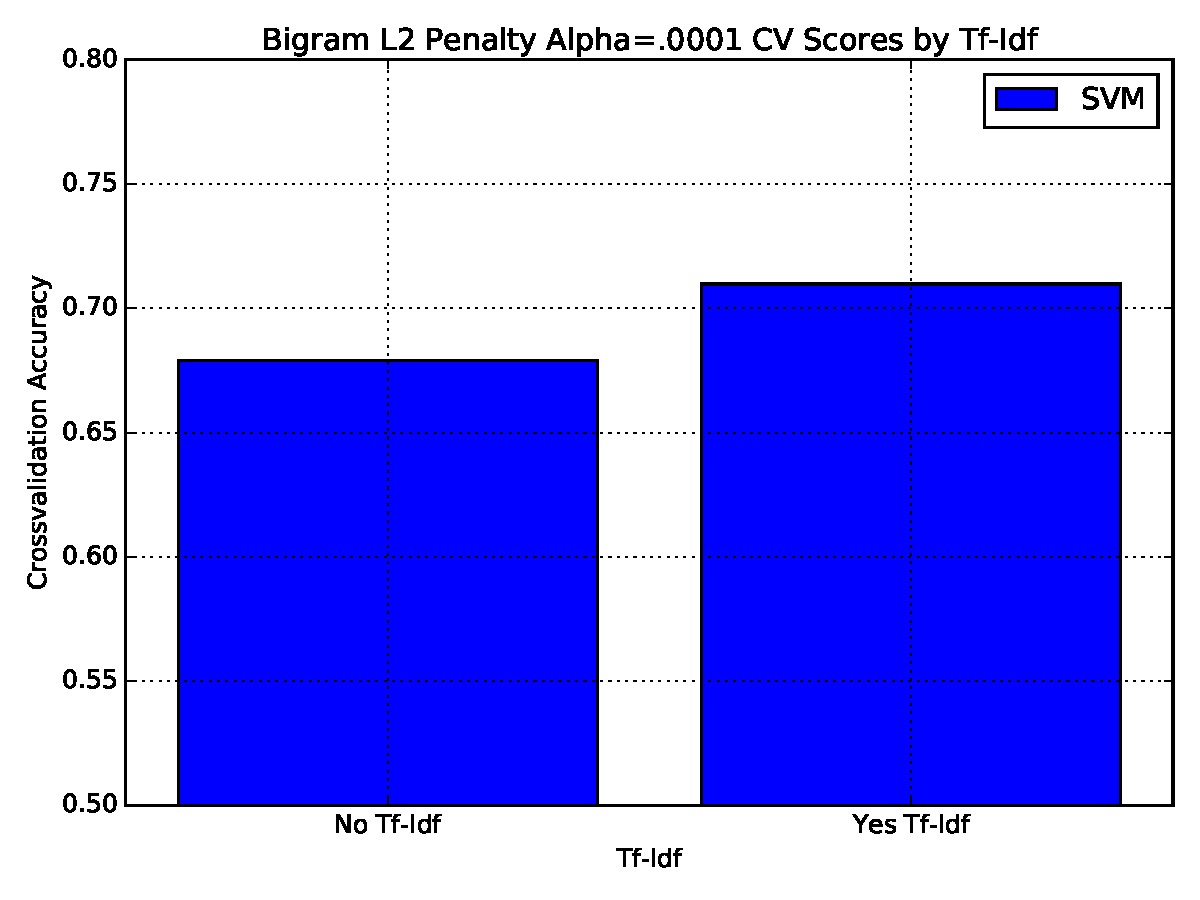
\includegraphics[width=\linewidth]{FiguresSVM_TFIDF_on_off_hinge.pdf}
\endminipage\hfill
\minipage{0.32\textwidth}
  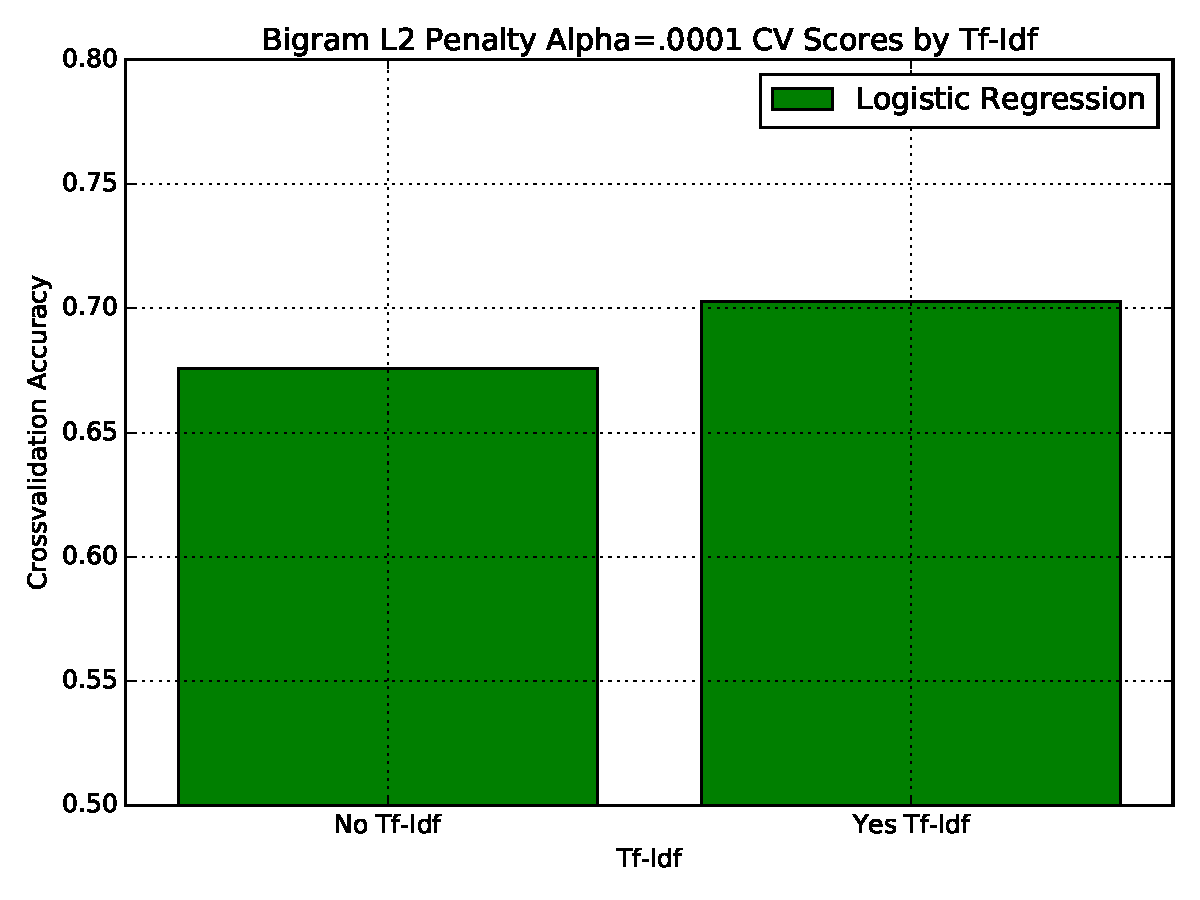
\includegraphics[width=\linewidth]{FiguresSVM_TFIDF_on_off_log.pdf}
\endminipage\hfill
\minipage{0.32\textwidth}
  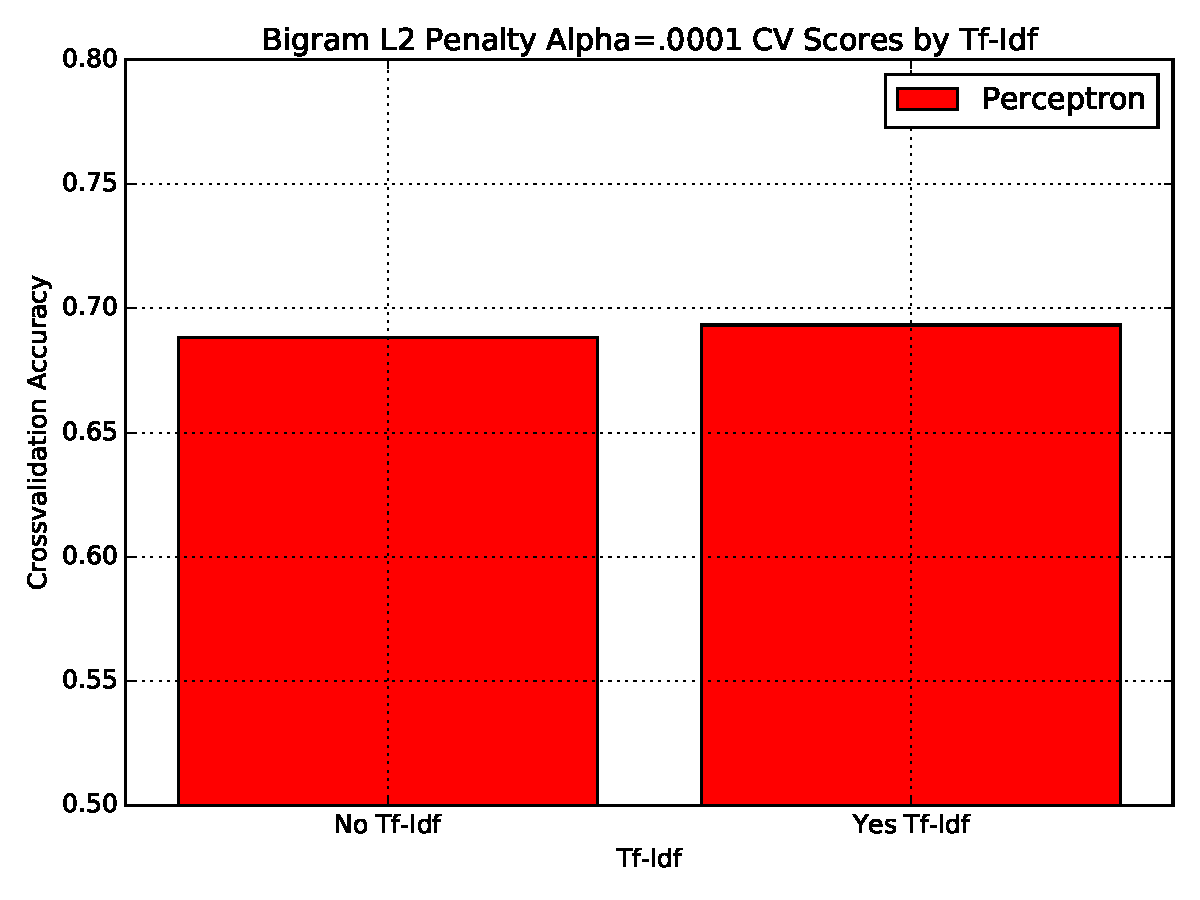
\includegraphics[width=\linewidth]{FiguresSVM_TFIDF_on_off_perceptron.pdf}
\endminipage
\caption[Tf-Idf On vs. Off for SGDClassifier with Varied Loss Functions]{Tf-Idf On vs. Off for SGDClassifier with Varied Loss Functions}
\label{fig: tfidf}
\end{figure}


\begin{figure}[!htb]
\minipage{0.32\textwidth}
  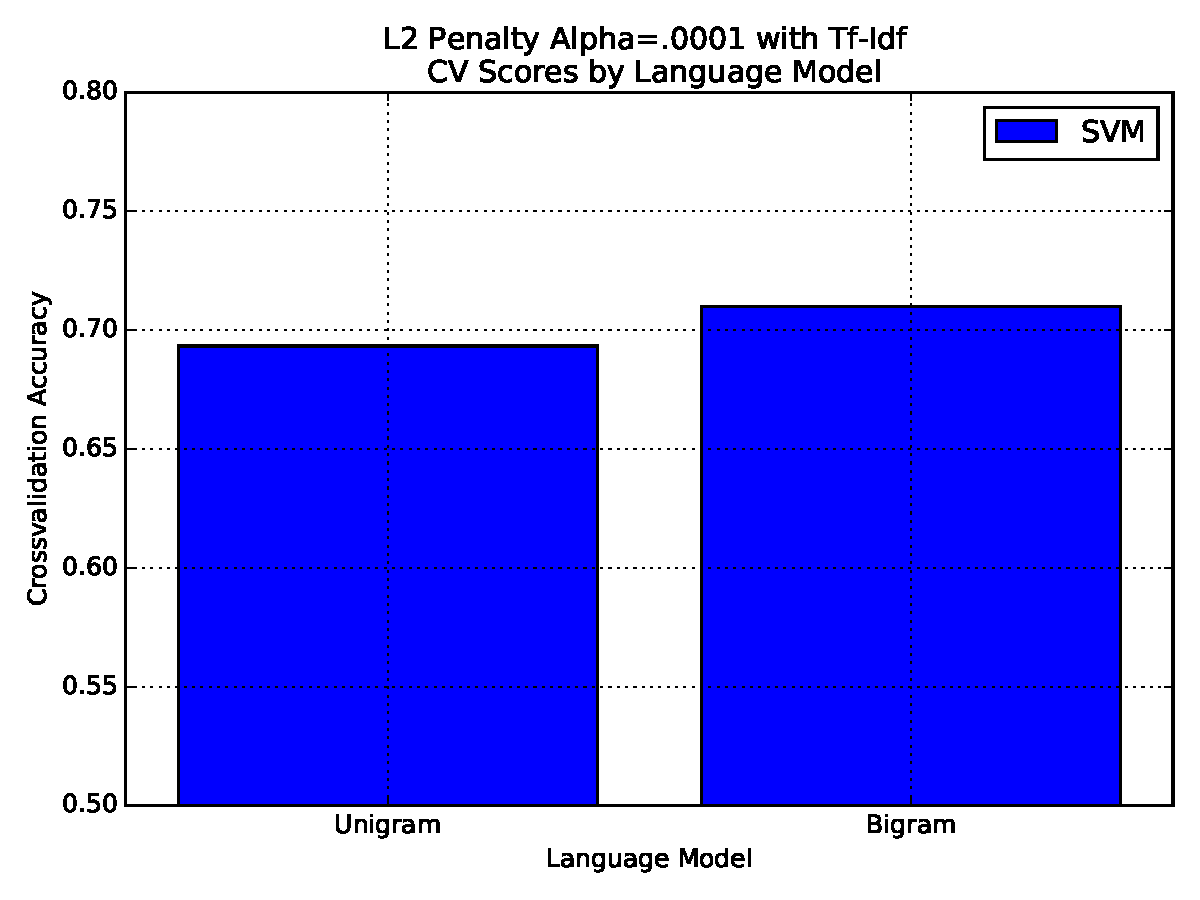
\includegraphics[width=\linewidth]{FiguresSVM_bigram_hinge.pdf}
\endminipage\hfill
\minipage{0.32\textwidth}
  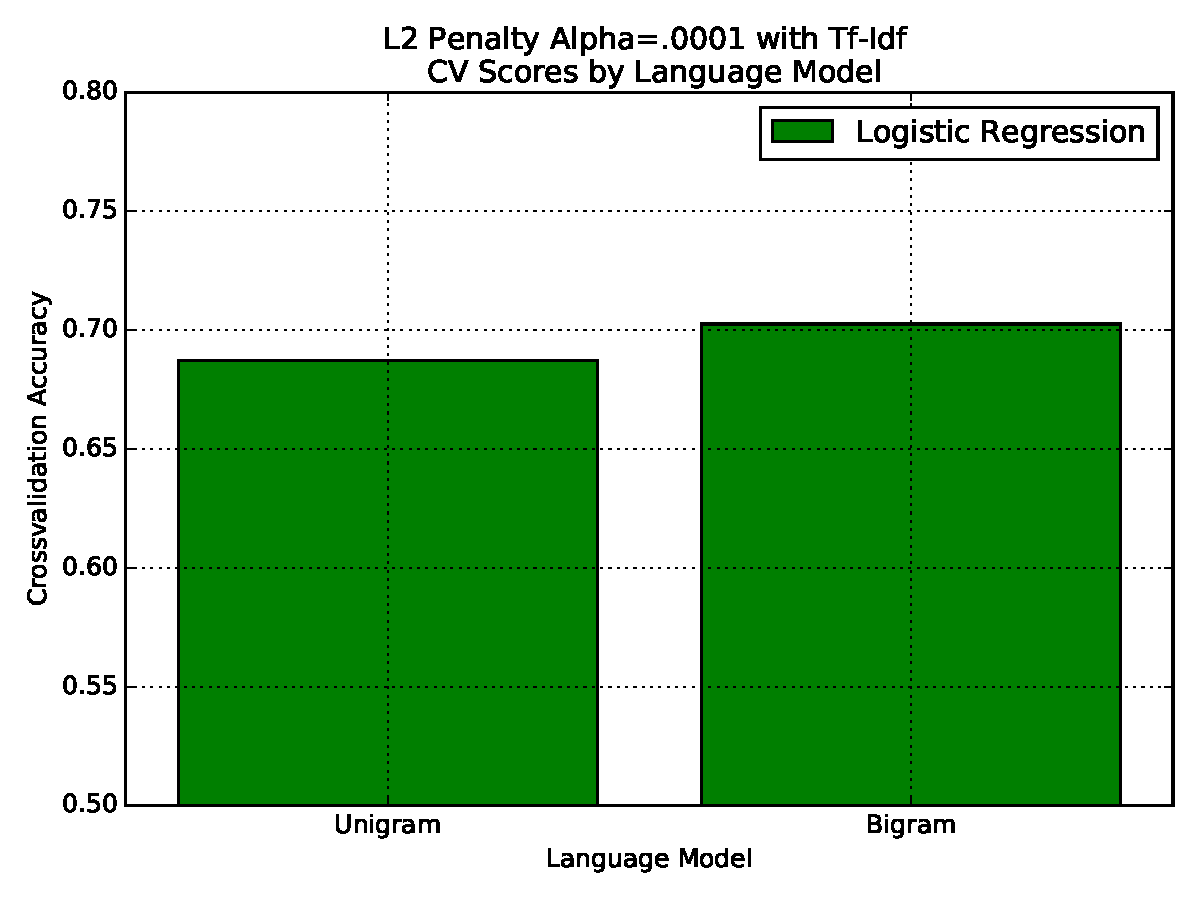
\includegraphics[width=\linewidth]{FiguresSVM_bigram_log.pdf}
\endminipage\hfill
\minipage{0.32\textwidth}
  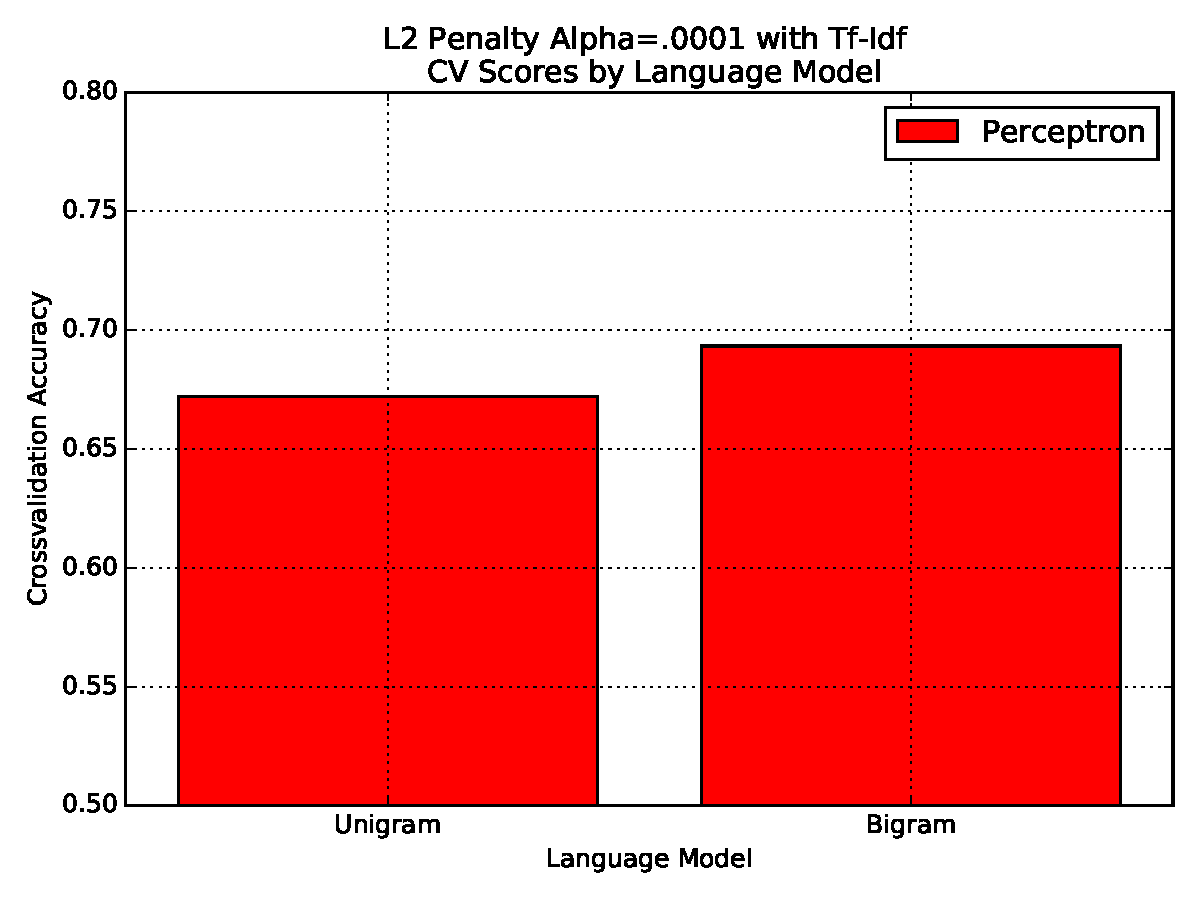
\includegraphics[width=\linewidth]{FiguresSVM_bigram_perceptron.pdf}
\endminipage
\caption[Unigram vs. Bigram for SGDClassifier with Varied Loss Functions]{Unigram vs. Bigram for SGDClassifier with Varied Loss Functions}
\label{fig: lm}
\end{figure}
\subsection{Optimal Hyper-parameters and Results}
For both Multinomial Naive Bayes and Stochastic Gradient Descent experiments we included Tf-Idf weighting and bigram language models. For Multinomial Naive Bayes we found an optimal $\alpha$ smoothing parameter at $\alpha=.05$ which resulted in a 3-fold cross-validation accuracy of 68.9\% and a test accuracy of 70.6\%. The Stochastic Gradient Descent classifier has many more hyper-parameters. The most important of these is the loss function because it determines the classification function. The Hinge loss function was found to be the most accurate in initial tests but we include the other loss functions in all cross-validation grid searches. While each loss function has its own set of optimal hyper-parameters, in general we find that the $l2$ norm penalty with a small regularization constant multiple $\alpha$ worked well with the Hinge loss function. We then searched a range of $\alpha$'s close to 0 as seen in \autoref{fig: sgd}. An optimal value of $\alpha=0.0001$ resulted in a 3-fold cross-validation accuracy of 70.9\% and a test accuracy of 74.8\%, which is the highest test accuracy we observed.

\begin{figure}[!ht]
\centering
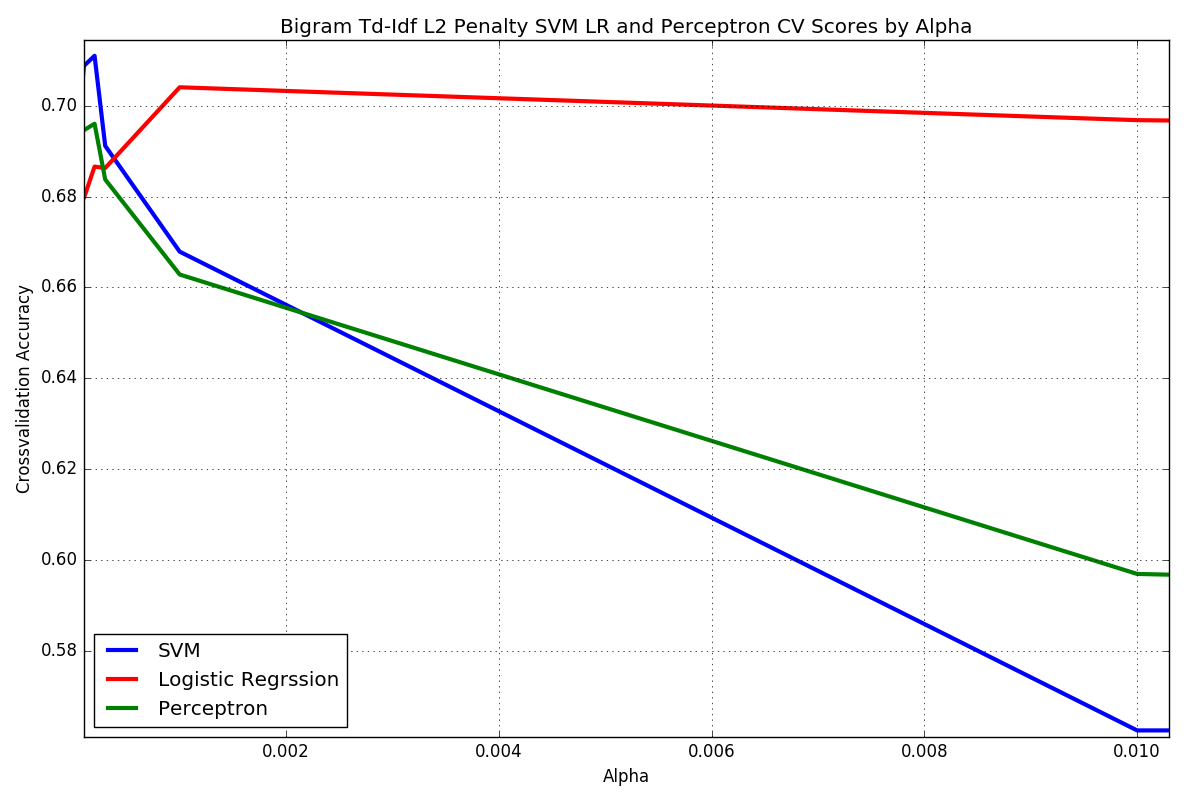
\includegraphics[width=0.5\linewidth]{ZoomedL2NormSVM.png}
\caption[SGDClassifier with Hinge Loss and $l2$ Penalty Over a Range of $\alpha$ ]{SGDClassifier with Hinge Loss and $l2$ Penalty Over Range of $\alpha$'s}
\label{fig: sgd}
\end{figure}

\section{Discussion and Future Work}
Overall our results seem to match those found in previous research. Thomas et al. note \cite{thomas2006get} that Support Vector Machines achieved the highest test accuracy of 71.2\% in predicting if a speaker would vote for or against a bill using this same corpus. This is similar to our result in that the Hinge loss function is the same used by Support Vector Machines and political party affiliation may be highly correlated with positions on a given bill.  Our higher accuracy may be do to many factors including our preforming a more exhaustive hyper-parameter search, or even the fact that not all votes are cast along party affiliation lines. That said, the fact that the same corpus is used and similar classification methods optimal results for both research questions is reassuring. An interesting future project to preform in the same vein as this research would be to test a recurrent neural network's performance, as mentioned by Iyyer \cite{iyyer2014political}, and see if accuracy increases. 
\newpage
\bibliographystyle{plain}
\bibliography{nlpFinal}
\end{document}